\documentclass[t,usenames,dvipsnames]{beamer}
\usetheme{Copenhagen}
\setbeamertemplate{headline}{} % remove toc from headers
\beamertemplatenavigationsymbolsempty

\usepackage{amsmath, tkz-euclide, tikz, xcolor, pgfplots, array}
\usetkzobj{all}
\pgfplotsset{compat = 1.16}
\usetikzlibrary{arrows.meta, calc, decorations.pathreplacing}
\pgfplotsset{every axis/.append style = {axis lines = middle, axis line style = {<->}}}
\pgfplotsset{every tick label/.append style={font=\tiny}}
\everymath{\displaystyle}

\title{Law of Sines and Law of Cosines}
\author{}
\date{}

\AtBeginSection[]
{
  \begin{frame}
    \frametitle{Objectives}
    \tableofcontents[currentsection]
  \end{frame}
}

\begin{document}

\begin{frame}
    \maketitle
\end{frame}

\section{Solve triangles using the Law of Sines}

\begin{frame}{Law of Sines}
    An \alert{oblique triangle} is one that does not contain a right angle. \newline\\
    
    To solve oblique, as well as right triangles, you can use either the Law of Sines or the Law of Cosines.
\end{frame}


\begin{frame}{Derivation of Law of Sines}
\begin{center}
\begin{tikzpicture}
\tkzDefPoints{0/0/A, 4/0/B, 2/2/C, 2/0/D}
\tkzDrawPolygon(A,B,C)
\tkzLabelPoints[left](A)
\tkzLabelPoints[above](C)
\tkzLabelPoints[right](B)
\tkzLabelSegment(A,C){b}
\tkzLabelSegment(B,C){a}
\tkzLabelSegment[below](A,B){c}
\onslide<2->{\tkzDrawSegment[red](C,D)}
\onslide<2->{\tkzLabelSegment[right,red](C,D){$y$}}
\end{tikzpicture}
\end{center}
\vspace{11pt}
\onslide<3->{
\begin{tabular}{p{0.6\textwidth}p{0.3\textwidth}}
    \begin{tikzpicture}
    \tkzDefPoints{0/0/A, 2/0/D/, 2/2/C}
    \tkzDrawPolygon(A,D,C)
    \tkzDrawSegment[color=red](C,D)
    \tkzLabelSegment[red,right](C,D){$y$}
    \tkzLabelSegment(A,C){b}
    \tkzLabelPoints[left](A)
    \tkzLabelPoints[above](C)
    \tkzLabelPoints[right](D)
    \end{tikzpicture} 
    &
    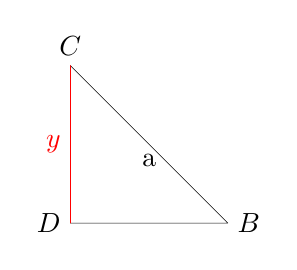
\begin{tikzpicture}
    \tkzDefPoints{0/0/D, 2/0/B, 0/2/C}
    \tkzDrawPolygon(B,D,C)
    \tkzDrawSegment[color=red](C,D)
    \tkzLabelSegment[red,left](C,D){$y$}
    \tkzLabelSegment(B,C){a}
    \tkzLabelPoints[right](B)
    \tkzLabelPoints[above](C)
    \tkzLabelPoints[left](D)
    \end{tikzpicture}
\end{tabular}}
\end{frame}

\begin{frame}{Derivation of Law of Sines}
\begin{tabular}{p{0.6\textwidth}p{0.3\textwidth}}
    \begin{tikzpicture}
    \tkzDefPoints{0/0/A, 2/0/D/, 2/2/C}
    \tkzDrawPolygon(A,D,C)
    \tkzDrawSegment[color=red](C,D)
    \tkzLabelSegment[red,right](C,D){$y$}
    \tkzLabelSegment(A,C){b}
    \tkzLabelPoints[left](A)
    \tkzLabelPoints[above](C)
    \tkzLabelPoints[right](D)
    \end{tikzpicture} 
    &
    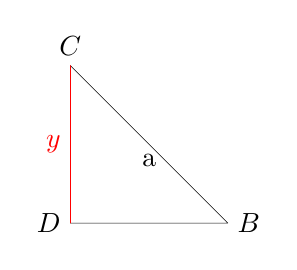
\begin{tikzpicture}
    \tkzDefPoints{0/0/D, 2/0/B, 0/2/C}
    \tkzDrawPolygon(B,D,C)
    \tkzDrawSegment[color=red](C,D)
    \tkzLabelSegment[red,left](C,D){$y$}
    \tkzLabelSegment(B,C){a}
    \tkzLabelPoints[right](B)
    \tkzLabelPoints[above](C)
    \tkzLabelPoints[left](D)
    \end{tikzpicture}
    \\[10pt]
    \onslide<2->{$\sin A = \frac{y}{b}$}  &   \onslide<4->{$\sin B = \frac{y}{a}$} \\
    \onslide<3->{$b\sin A = y$}           &   \onslide<5->{$a\sin B = y$}   \\
\end{tabular}
\begin{align*}
    \onslide<6->{b\sin A &= a\sin B}
\end{align*}
\end{frame}

\begin{frame}{Derivation of Law of Sines}
    \begin{align*}
        b\sin A &= a\sin B \\[10pt]
        \onslide<2->{\frac{b\sin A}{ab} &= \frac{a\sin B}{ab}} \\[10pt]
        \onslide<3->{\frac{\sin A}{a} &= \frac{\sin B}{b}}
    \end{align*}
    \onslide<4->{{\color{red}\[\frac{\sin A}{a} = \frac{\sin B}{b} = \frac{\sin C}{c}\]}}
\end{frame}

\begin{frame}{Example 1}
Solve the triangle given $m\angle A = 120^\circ, \, a = 7, \, m\angle B = 45^\circ$. Round your answers to 1 decimal place.   \newline\\
\begin{minipage}{0.5\textwidth}
\begin{tikzpicture}[scale=0.95]
\tkzDefPoints{0/0/B, 2/2/A, 4/0/C}
\tkzDrawPolygon(A,B,C)
\tkzLabelPoints[above](A)
\tkzLabelPoints[left](B)
\tkzLabelPoints[right](C)
\tkzLabelAngle[pos=0.7](C,B,A){$45^\circ$}
\tkzLabelAngle[pos=0.5](C,A,B){$120^\circ$}
\tkzLabelSegment[below](B,C){7}
\end{tikzpicture}
\end{minipage}
\begin{minipage}{0.4\textwidth}
\onslide<2->{$m\angle C = 180^\circ - 120^\circ - 45^\circ$}  \\[15pt]
\onslide<3->{$m\angle C = 15^\circ$}
\end{minipage}
\end{frame}

\begin{frame}{Example 1}
\begin{minipage}{0.5\textwidth}
\begin{tikzpicture}[scale=0.95]
\tkzDefPoints{0/0/B, 2/2/A, 4/0/C}
\tkzDrawPolygon(A,B,C)
\tkzLabelPoints[above](A)
\tkzLabelPoints[left](B)
\tkzLabelPoints[right](C)
\tkzLabelAngle[pos=0.7](C,B,A){$45^\circ$}
\tkzLabelAngle[pos=0.5](C,A,B){$120^\circ$}
\tkzLabelAngle[pos=0.7, color=red](B,C,A){$15^\circ$}
\tkzLabelSegment[below](B,C){7}
\end{tikzpicture}
\end{minipage}    
\begin{minipage}{0.4\textwidth}
\begin{align*}
    \onslide<2->{\frac{\sin 120^\circ}{7} &= \frac{\sin 45^\circ}{b}} \\[12pt]
    \onslide<3->{b\sin 120^\circ &= 7\sin 45^\circ} \\[12pt]
    \onslide<4->{b &= \frac{7\sin 45^\circ}{\sin 120^\circ}} \\[12pt]
    \onslide<5->{b &\approx 5.7}
\end{align*}
\end{minipage}
\end{frame}

\begin{frame}{Example 1}
\begin{minipage}{0.5\textwidth}
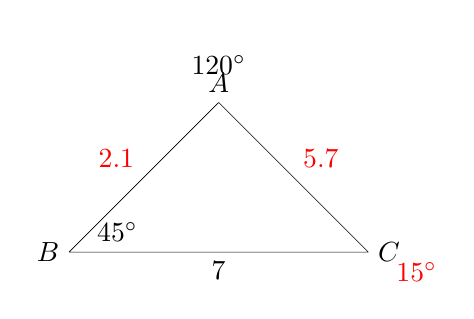
\begin{tikzpicture}[scale=0.95]
\tkzDefPoints{0/0/B, 2/2/A, 4/0/C}
\tkzDrawPolygon(A,B,C)
\tkzLabelPoints[above](A)
\tkzLabelPoints[left](B)
\tkzLabelPoints[right](C)
\tkzLabelAngle[pos=0.7](C,B,A){$45^\circ$}
\tkzLabelAngle[pos=0.5](C,A,B){$120^\circ$}
\tkzLabelAngle[pos=0.7, color=red](B,C,A){$15^\circ$}
\tkzLabelSegment[color=red,above right](A,C){$5.7$}
\tkzLabelSegment[below](B,C){7}
\onslide<6->{\tkzLabelSegment[color=red,above left](A,B){$2.1$}}
\end{tikzpicture}
\end{minipage}    
\begin{minipage}{0.4\textwidth}
\begin{align*}
    \onslide<2->{\frac{\sin 120^\circ}{7} &= \frac{\sin 15^\circ}{c}} \\[12pt]
    \onslide<3->{c\sin 120^\circ &= 7\sin 15^\circ} \\[12pt]
    \onslide<4->{c &= \frac{7\sin 15^\circ}{\sin 120^\circ}} \\[12pt]
    \onslide<5->{c &\approx 2.1}
\end{align*}
\end{minipage}
\vspace{11pt}
\[\onslide<7->{m\angle C = 15^\circ, \quad b \approx 5.7, \quad c \approx 2.1}\]
\end{frame}

\begin{frame}{Example 2}
Solve the triangle given $m\angle A = 85^\circ, \, m\angle B = 30^\circ, \, c = 5.25$   \newline\\  
\begin{minipage}{0.5\textwidth}
\onslide<2->{
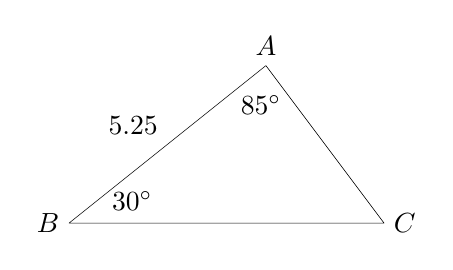
\begin{tikzpicture}
\tkzDefPoints{0/0/B, 4/0/C, 2.5/2/A}
\tkzDrawPolygon(A,B,C)
\tkzLabelPoints[right](C)
\tkzLabelPoints[left](B)
\tkzLabelPoints[above](A)
\tkzLabelSegment[above left](B,A){5.25}
\tkzLabelAngle[pos=0.5](B,A,C){$85^\circ$}
\tkzLabelAngle[pos=0.85](C,B,A){$30^\circ$}
\end{tikzpicture}}
\end{minipage}
\begin{minipage}{0.4\textwidth}
\onslide<3->{$m\angle C = 180^\circ - 30^\circ - 85^\circ$} \\[12pt]
\onslide<4->{$m\angle C = 65^\circ$}
\end{minipage}
\end{frame}

\begin{frame}{Example 2}
\begin{minipage}{0.5\textwidth}
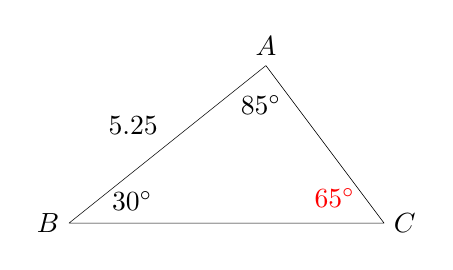
\begin{tikzpicture}
\tkzDefPoints{0/0/B, 4/0/C, 2.5/2/A}
\tkzDrawPolygon(A,B,C)
\tkzLabelPoints[right](C)
\tkzLabelPoints[left](B)
\tkzLabelPoints[above](A)
\tkzLabelSegment[above left](B,A){5.25}
\tkzLabelAngle[pos=0.5](B,A,C){$85^\circ$}
\tkzLabelAngle[pos=0.85](C,B,A){$30^\circ$}
\tkzLabelAngle[pos=0.7,color=red](A,C,B){$65^\circ$}
\end{tikzpicture}
\end{minipage}
\begin{minipage}{0.4\textwidth}
\begin{align*}
    \onslide<2->{\frac{\sin 65^\circ}{5.25} &= \frac{\sin 85^\circ}{a}} \\[12pt]
    \onslide<3->{a\cdot \sin65^\circ &= 5.25\sin 85^\circ} \\[12pt]
    \onslide<4->{a &= \frac{5.25\sin 85^\circ}{\sin 65^\circ}} \\[12pt]
    \onslide<5->{a &\approx 5.8}
\end{align*}
\end{minipage}
\end{frame}

\begin{frame}{Example 2}
\begin{minipage}{0.5\textwidth}
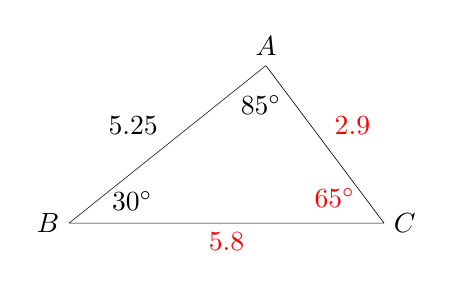
\begin{tikzpicture}
\tkzDefPoints{0/0/B, 4/0/C, 2.5/2/A}
\tkzDrawPolygon(A,B,C)
\tkzLabelPoints[right](C)
\tkzLabelPoints[left](B)
\tkzLabelPoints[above](A)
\tkzLabelSegment[above left](B,A){5.25}
\tkzLabelAngle[pos=0.5](B,A,C){$85^\circ$}
\tkzLabelAngle[pos=0.85](C,B,A){$30^\circ$}
\tkzLabelAngle[pos=0.7,color=red](A,C,B){$65^\circ$}
\tkzLabelSegment[below,red](B,C){5.8}
\onslide<6->{\tkzLabelSegment[red, above right](A,C){2.9}}
\end{tikzpicture}
\end{minipage}
\begin{minipage}{0.4\textwidth}
\begin{align*}
    \onslide<2->{\frac{\sin 65^\circ}{5.25} &= \frac{\sin 30^\circ}{b}} \\[12pt]
    \onslide<3->{b\cdot \sin65^\circ &= 5.25\sin 30^\circ} \\[12pt]
    \onslide<4->{b &= \frac{5.25\sin 30^\circ}{\sin 65^\circ}} \\[12pt]
    \onslide<5->{b &\approx 2.9}
\end{align*}
\end{minipage}  \vspace{11pt}
\[
\onslide<7->{m\angle C = 65^\circ, \quad a \approx 5.8, \quad b \approx 2.9}
\]
\end{frame}

\section{Solve triangles using the Law of Cosines}

\begin{frame}{Derivation of the Law of Cosines}
\begin{center}
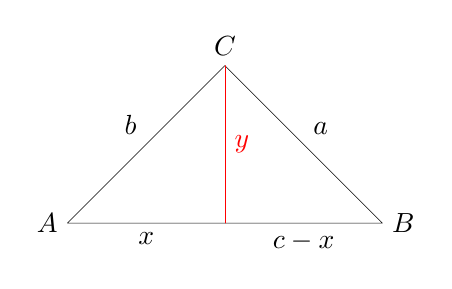
\begin{tikzpicture}
\tkzDefPoints{0/0/A, 4/0/B, 2/2/C, 2/0/D}
\tkzDrawPolygon(A,B,C)
\tkzLabelPoints[left](A)
\tkzLabelPoints[above](C)
\tkzLabelPoints[right](B)
\tkzLabelSegment[above left](A,C){$b$}
\tkzLabelSegment[above right](C,B){$a$}
\onslide<2->{\tkzDrawSegment[red](C,D)
\tkzLabelSegment[red,right](C,D){$y$}
\tkzLabelSegment[below](A,D){$x$}
\tkzLabelSegment[below](B,D){$c-x$}
}
\end{tikzpicture}
\end{center}
\begin{align*}
    \onslide<3->{x^2 + {\color{red}y}^2 &= b^2 & (c-x)^2 + {\color{red}y}^2 = a^2} \\[6pt]
    \onslide<4->{{\color{red}y}^2 &= b^2 - x^2 & c^2 - 2cx + x^2 + {\color{red}y}^2 &= a^2}
\end{align*}
\begin{align*}
    \onslide<5->{c^2 - 2cx + x^2 + {\color{red}b^2 - x^2} &= a^2} \\
    \onslide<6->{b^2 + c^2 - 2cx &= a^2}
\end{align*}
\end{frame}

\begin{frame}{Derivation of Law of Cosines}
\begin{center}
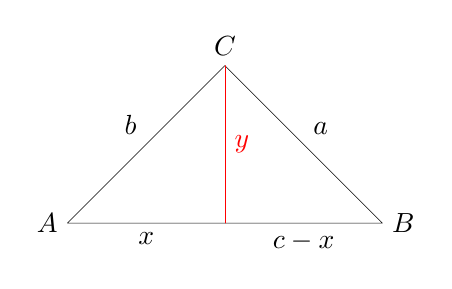
\begin{tikzpicture}
\tkzDefPoints{0/0/A, 4/0/B, 2/2/C, 2/0/D}
\tkzDrawPolygon(A,B,C)
\tkzLabelPoints[left](A)
\tkzLabelPoints[above](C)
\tkzLabelPoints[right](B)
\tkzLabelSegment[above left](A,C){$b$}
\tkzLabelSegment[above right](C,B){$a$}
\tkzDrawSegment[red](C,D)
\tkzLabelSegment[red,right](C,D){$y$}
\tkzLabelSegment[below](A,D){$x$}
\tkzLabelSegment[below](B,D){$c-x$}
\end{tikzpicture}
\end{center}
\begin{align*}
    \onslide<2->{a^2 &= b^2 + c^2 - 2cx} \\
    \onslide<3->{\cos A &= \frac{x}{b}} \\[6pt]
    \onslide<4->{x &= b\cos A} \\[6pt]
    \onslide<5->{a^2 &= b^2 + c^2 - 2c(b\cos A)}
\end{align*}
\end{frame}

\begin{frame}{Law of Cosines}
    \begin{align*}
        a^2 &= b^2 + c^2 - 2bc(\cos A) \\[12pt]
        b^2 &= a^2 + c^2 - 2ac(\cos B) \\[12pt]
        c^2 &= a^2 + b^2 - 2ab(\cos C)
    \end{align*}
\end{frame}

\begin{frame}{Law of Cosines}
By solving each of the previous equations for the cosine of the angle, we get the following:
\begin{align*}
    \cos A &= \frac{b^2+c^2-a^2}{2bc}   \\[12pt]
    \cos B &= \frac{a^2+c^2-b^2}{2ac}   \\[12pt]
    \cos C &= \frac{a^2+b^2-c^2}{2ab}   \\[12pt]
\end{align*}
Then take the inverse cosine to get the angle measure.
\end{frame}

\begin{frame}{Example 3}
Solve each. Round your answers to one decimal place.    \newline\\
$m\angle A = 60^\circ, \, b = 20, \, c = 30$    \newline\\
\begin{minipage}{0.5\textwidth}
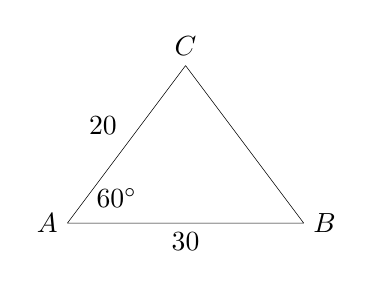
\begin{tikzpicture}
\tkzDefPoints{0/0/A, 3/0/B/, 1.5/2/C}
\tkzDrawPolygon(A,B,C)
\tkzLabelPoints[left](A)
\tkzLabelPoints[above](C)
\tkzLabelPoints[right](B)
\tkzLabelAngle[pos=0.7](B,A,C){$60^\circ$}
\tkzLabelSegment[below](A,B){30}
\tkzLabelSegment[above left](A,C){20}
\end{tikzpicture}
\end{minipage}
\hspace{-0.5cm}
\begin{minipage}{0.4\textwidth}
\begin{align*}
    \onslide<2->{a^2 &= 20^2 + 30^2 - 2(20)(30)\cos60^\circ} \\[12pt]
    \onslide<3->{a^2 &= 700} \\[12pt]
    \onslide<4->{a &\approx 26.5}
\end{align*}
\end{minipage}
\end{frame}

\begin{frame}{Example 3}
\begin{minipage}{0.5\textwidth}
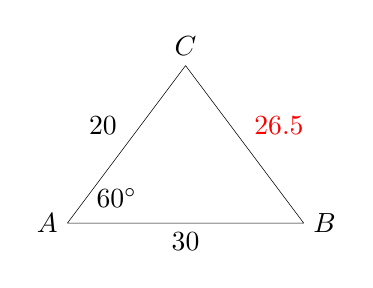
\begin{tikzpicture}
\tkzDefPoints{0/0/A, 3/0/B/, 1.5/2/C}
\tkzDrawPolygon(A,B,C)
\tkzLabelPoints[left](A)
\tkzLabelPoints[above](C)
\tkzLabelPoints[right](B)
\tkzLabelAngle[pos=0.7](B,A,C){$60^\circ$}
\tkzLabelSegment[below](A,B){30}
\tkzLabelSegment[above left](A,C){20}
\tkzLabelSegment[above right, red](B,C){26.5}
\end{tikzpicture}
\end{minipage}
\hspace{-0.5cm}
\begin{minipage}{0.4\textwidth}
\begin{align*}
    \onslide<2->{\cos B &= \frac{26.5^2 + 30^2 - 20^2}{2(26.5)(30)}} \\[12pt]
    \onslide<3->{\cos B &\approx 0.7561} \\[12pt]
    \onslide<4->{B &\approx 40.9^\circ} 
\end{align*}
\end{minipage}
\end{frame}


\begin{frame}{Example 3}
\begin{minipage}{0.5\textwidth}
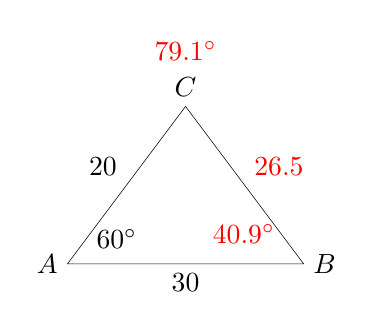
\begin{tikzpicture}
\tkzDefPoints{0/0/A, 3/0/B/, 1.5/2/C}
\tkzDrawPolygon(A,B,C)
\tkzLabelPoints[left](A)
\tkzLabelPoints[above](C)
\tkzLabelPoints[right](B)
\tkzLabelAngle[pos=0.7](B,A,C){$60^\circ$}
\tkzLabelSegment[below](A,B){30}
\tkzLabelSegment[above left](A,C){20}
\tkzLabelSegment[above right, red](B,C){26.5}
\onslide<4->{\tkzLabelAngle[color=red,pos=0.7](B,C,A){$79.1^\circ$}}
\tkzLabelAngle[color=red,pos=0.85](C,B,A){$40.9^\circ$}
\end{tikzpicture}
\end{minipage}
\hspace{-0.5cm}
\begin{minipage}{0.4\textwidth}
\begin{align*}
    \onslide<2->{m\angle C &\approx 180^\circ - 60^\circ - 40.9^\circ} \\[12pt]
    \onslide<3->{m\angle C &\approx 79.1^\circ}
\end{align*}
\end{minipage}
\onslide<5->{\[a \approx 26.5, \quad m\angle B \approx 40.9^\circ, \quad m\angle C \approx 79.1^\circ \]}
\end{frame}

\begin{frame}{Example 4}
Solve the triangle. Round your answers to 1 decimal place.  \newline\\
$a = 6, \, b = 9, \, c = 4$ \newline\\
\begin{minipage}{0.5\textwidth}
\begin{tikzpicture}
\tkzDefPoints{0/0/A, 3/0/C, 1/1.75/B}
\tkzLabelPoints[left](A)
\tkzLabelPoints[above](B)
\tkzLabelPoints[right](C)
\tkzDrawPolygon(A,B,C)
\tkzLabelSegment[below](A,C){9}
\tkzLabelSegment[above left](A,B){4}
\tkzLabelSegment[above right](B,C){6}
\end{tikzpicture}
\end{minipage}
\begin{minipage}{0.4\textwidth}
\begin{align*}
\onslide<2->{\cos A &= \frac{9^2 + 4^2 - 6^2}{2(9)(4)}} \\[12pt]
\onslide<3->{\cos A &= \frac{61}{72}} \\[12pt]
\onslide<4->{A &\approx 32.1^\circ}
\end{align*}
\end{minipage}
\end{frame}


\begin{frame}{Example 4}
\begin{minipage}{0.5\textwidth}
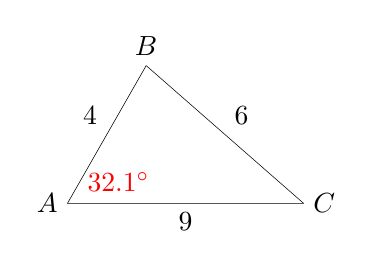
\begin{tikzpicture}
\tkzDefPoints{0/0/A, 3/0/C, 1/1.75/B}
\tkzLabelPoints[left](A)
\tkzLabelPoints[above](B)
\tkzLabelPoints[right](C)
\tkzDrawPolygon(A,B,C)
\tkzLabelSegment[below](A,C){9}
\tkzLabelSegment[above left](A,B){4}
\tkzLabelSegment[above right](B,C){6}
\tkzLabelAngle[pos=0.75,color=red, yshift=-0.1cm](C,A,B){$32.1^\circ$}
\end{tikzpicture}
\end{minipage}
\begin{minipage}{0.4\textwidth}
\begin{align*}
\onslide<2->{\cos B &= \frac{6^2 + 4^2 - 9^2}{2(6)(4)}} \\[12pt]
\onslide<3->{\cos B &= -\frac{29}{48}} \\[12pt]
\onslide<4->{B &\approx 127.2^\circ}
\end{align*}
\end{minipage}
\end{frame}


\begin{frame}{Example 4}
\begin{minipage}{0.5\textwidth}
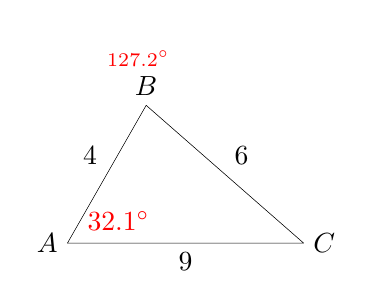
\begin{tikzpicture}
\tkzDefPoints{0/0/A, 3/0/C, 1/1.75/B}
\tkzLabelPoints[left](A)
\tkzLabelPoints[above](B)
\tkzLabelPoints[right](C)
\tkzDrawPolygon(A,B,C)
\tkzLabelSegment[below](A,C){9}
\tkzLabelSegment[above left](A,B){4}
\tkzLabelSegment[above right](B,C){6}
\tkzLabelAngle[pos=0.75,color=red, yshift=-0.1cm](C,A,B){$32.1^\circ$}
\tkzLabelAngle[pos=0.6,color=red](C,B,A){\scriptsize $127.2^\circ$}
\end{tikzpicture}
\end{minipage}
\begin{minipage}{0.4\textwidth}
\begin{align*}
\onslide<2->{m\angle C &\approx 180^\circ - 127.2^\circ - 32.1^\circ}   \\[12pt]
\onslide<3->{m\angle C &\approx 20.7^\circ}
\end{align*}
\end{minipage}
\onslide<4->{\[m\angle A \approx 32.1^\circ, \quad m\angle B \approx 127.2^\circ, \quad m\angle C \approx 20.7^\circ\]}
\end{frame}

\end{document}
